\begin{abstract}
Количество доступных трехмерных структур биомолекул постоянно увеличивается и современная биохимическая работа все чаще требует не только <<мокрых>> экспериментов, но и анализа структуры изучаемого объекта. При этом, наглядное представление трехмерных объектов на бумаге~-- задача не всегда тривиальная. Хорошая картинка может существенно сократить текст статьи, а плохая~-- наоборот, запутать читателя. 
\end{abstract}

Практический семинар <<Визуализация структур в UCSF Chimera>> длительностью 2 академических часа поможет студентам научиться подготавливать качественные иллюстрации для научных работ. На семинаре будут рассмотрены основные приемы работы с программой UCSF Chimera\footnote{\url{https://www.cgl.ucsf.edu/chimera/}}:
\begin{enumerate}
    \item различные форматы файлов со структурами белков и ДНК; % +
    \item где их можно получить и как открыть в химере; % +
    \item освещение (одно-, двух- и трехточечное, изотропное), цвет фона; % +
    \item способы отображения биомолекул (полноатомный, \textit{ribbon}, поверхности); % +
    \item выделение элементов структуры, именованные группы атомов, отображение/скрытие элементов структуры; % +
    \item структурное выравнивание; % +
    \item раскраска: по атрибутам, радуга; %+
    \item поиск водородных связей и межатомных контактов, построение поверхностей \textit{SAS, SES} и \textit{VdW}; %+
    \item прозрачность, сечения и вид в разрезе; %+
    \item сохранение полученной иллюстрации, виды доступной трассировки лучей.
\end{enumerate}
\hfill
\begin{figure}[h!]
  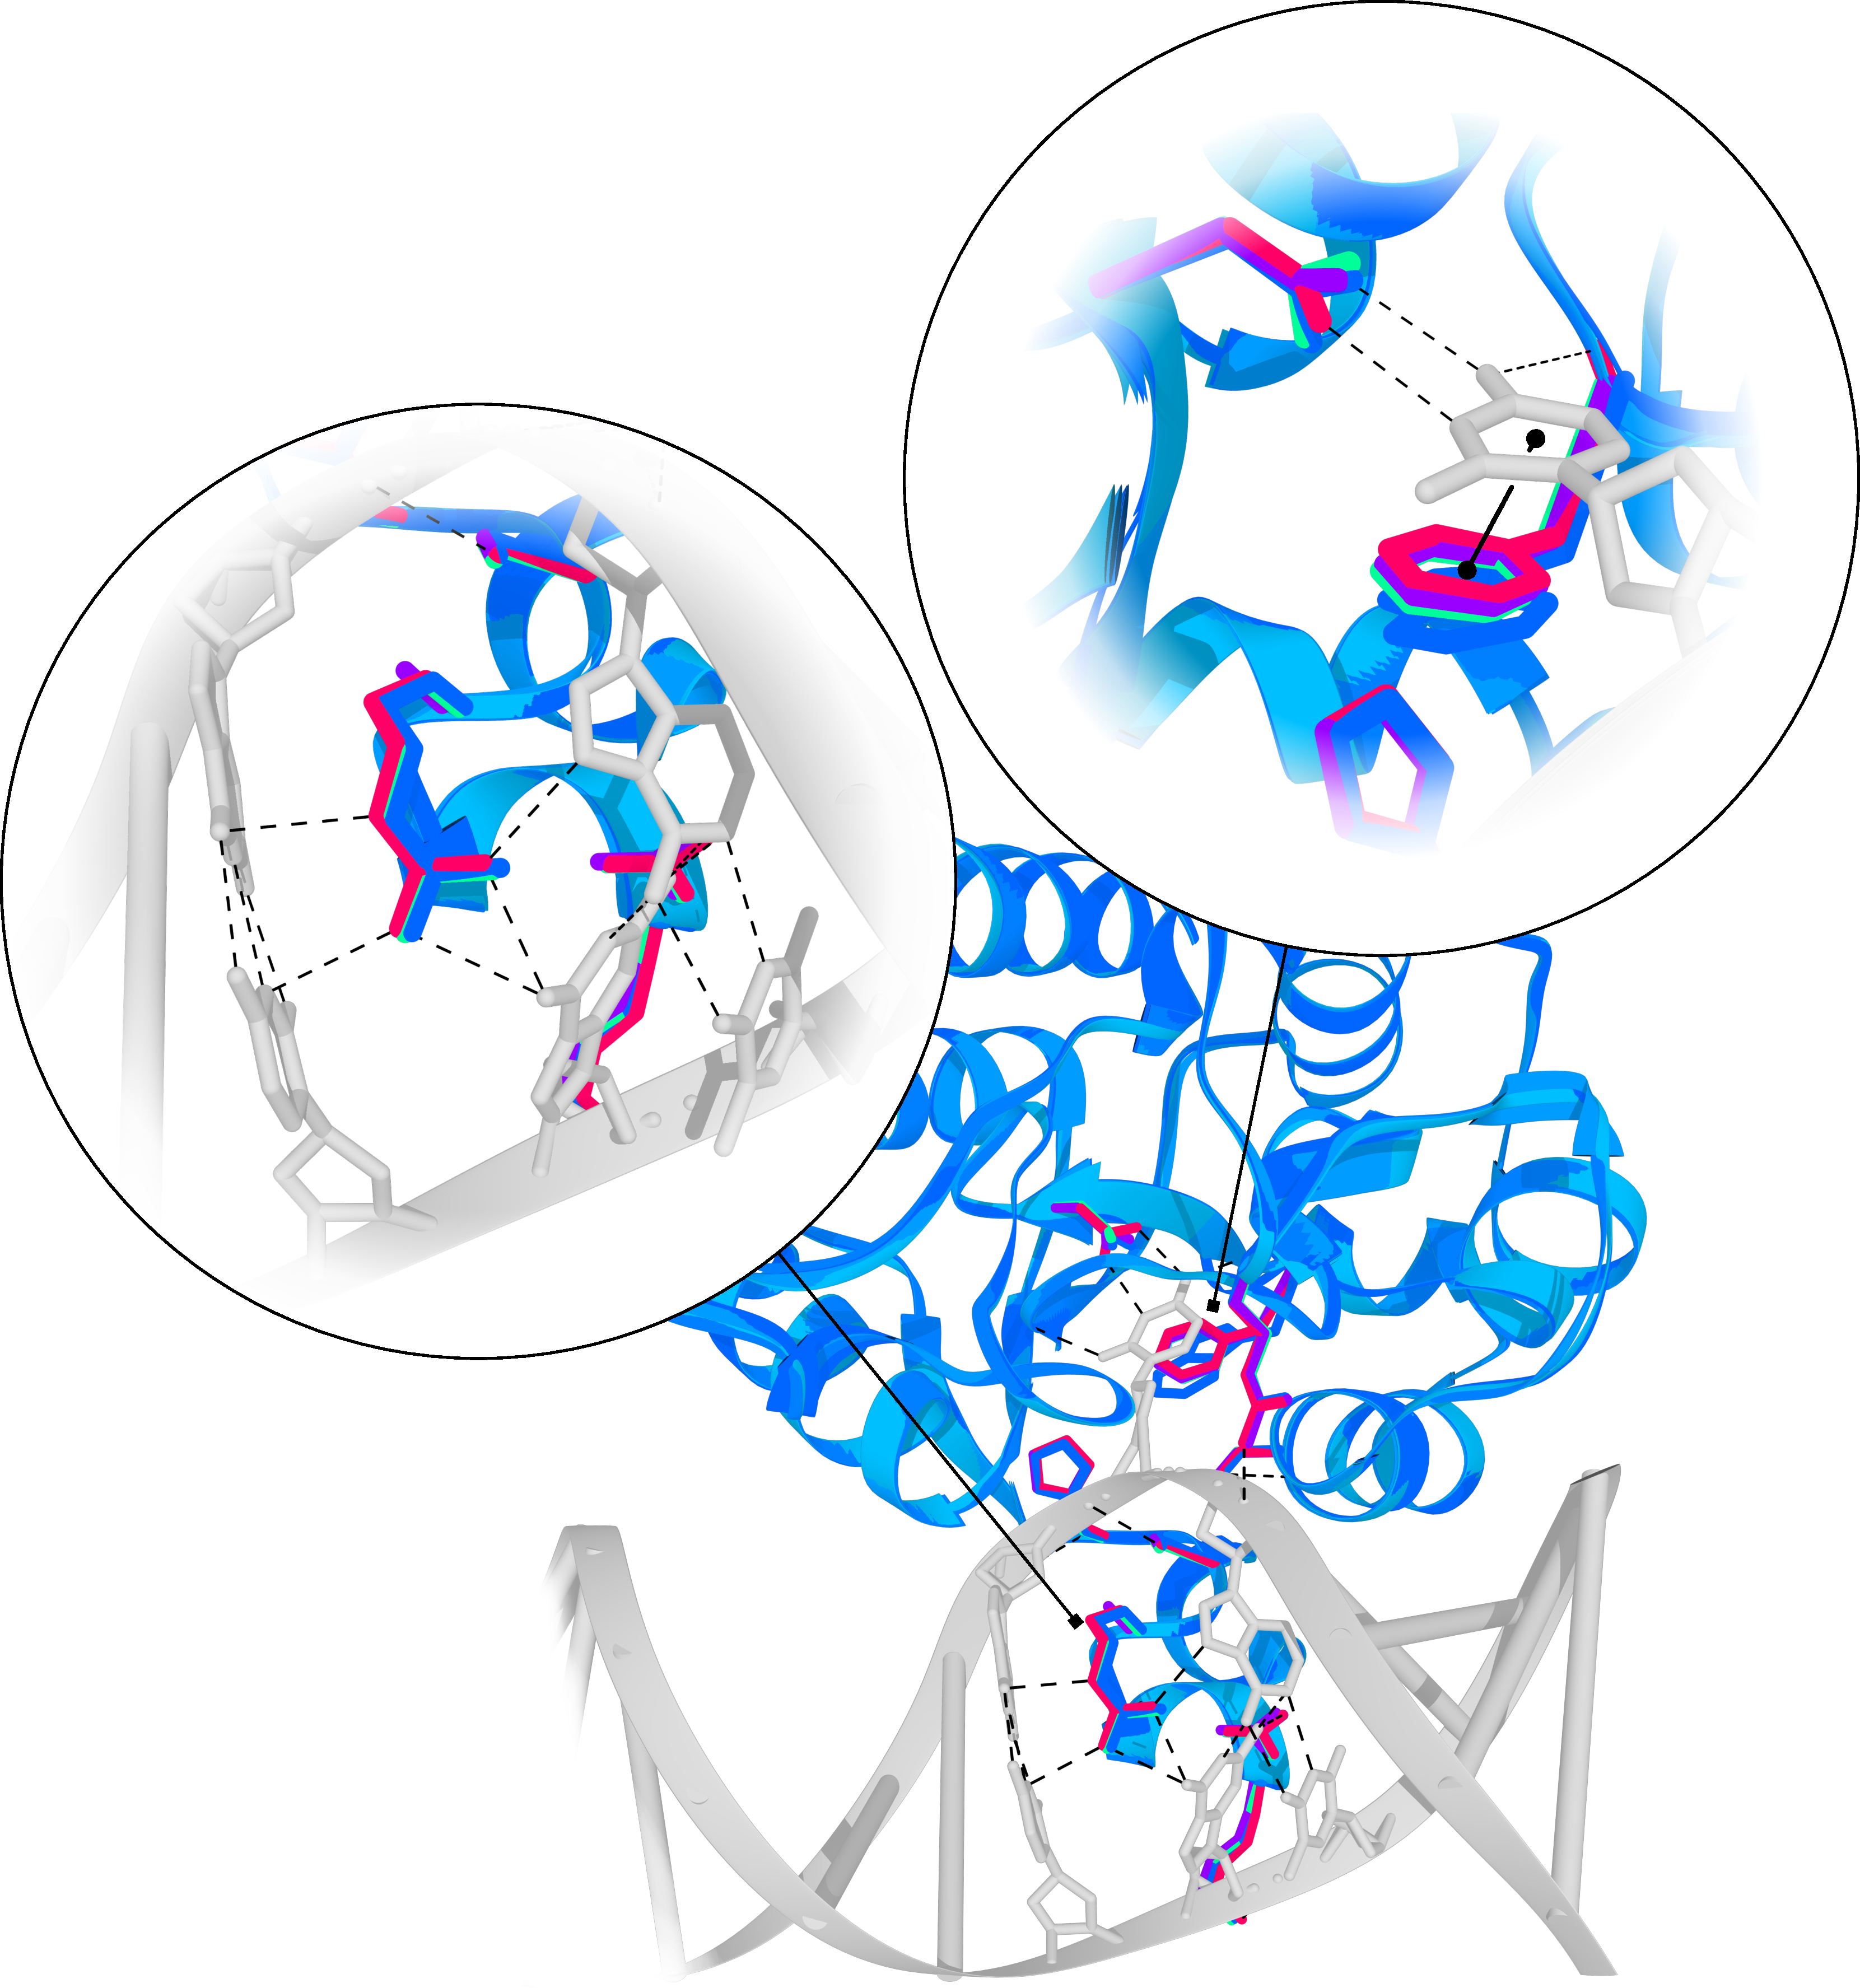
\includegraphics[width=\linewidth]{Figures/Protein.pdf}
  \caption{\textit{Пример иллюстрации подготовленной с помощью UCSF Chimera.}}
  \label{fig:smug}
\end{figure}